\section{Aufbau}
\label{sec:Aufbau}

Der Versuchsaufbau ist in Abbildung \ref{fig:aufbau} dargestellt.
\begin{figure}
  \centering
  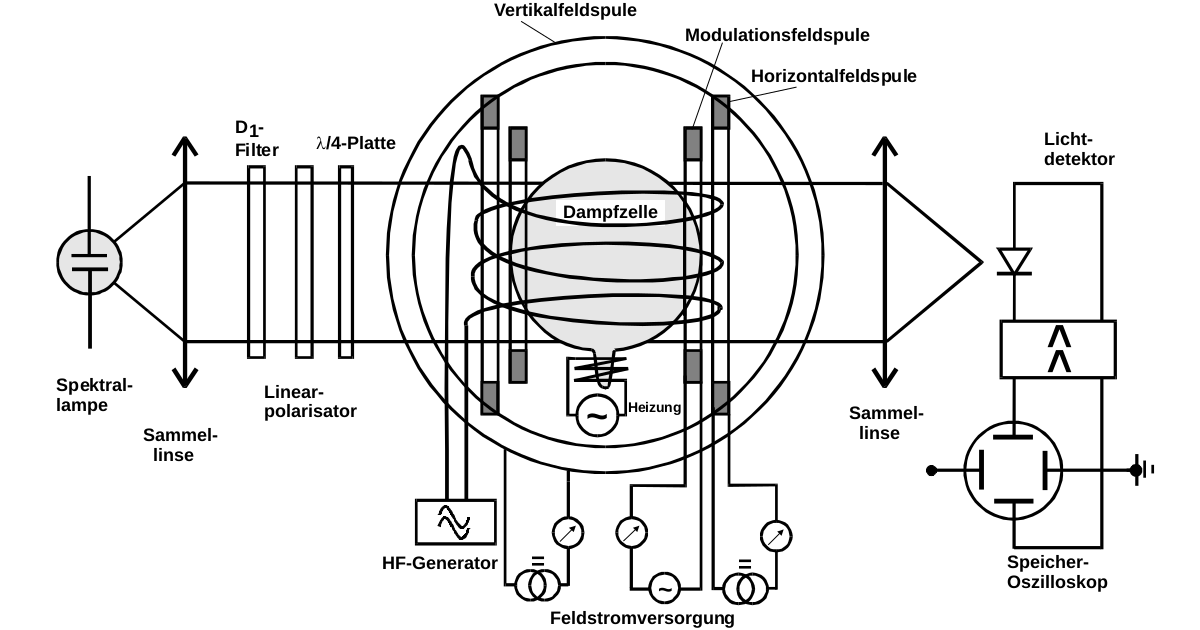
\includegraphics[height=8.5cm]{ressources/versuch.png}
  \caption{Versuchsaufbau zum optischen Pumpen (von oben) \cite{skript}.}
  \label{fig:aufbau}
\end{figure}
Dessen Kernelement bildet eine Dampfzelle, welche mit den Rubidium-Isotopen $^{85}$Rb und $^{87}$Rb gefüllt ist.
Am Anfang der Versuchsapparatur steht eine Spektrallampe.
Der dadurch emittierte Lichtstrahl wird zunächst durch eine Sammellinse aufgebreitet.
Darauf folgt ein D$_1$-Filter, welcher nur die D$_1$-Linie des Rubidium-Spektrums ($\lambda = \SI{794.8}{\nano\meter}$) durchlässt.
Anschließend durchläuft der Lichtstrahl einen Linearpolarisator und eine $\lambda/4$-Platte, um zirkularpolarisiertes Licht zu erzeugen.
Das Licht passiert die Dampfzelle und wird danach durch eine weitere Sammellinse auf ein SI-Photoelement fokussiert, welches über einen Linearverstärker an dem Y-Eingang eines Oszilloskops angeschlossen ist.
Das Gas in der Dampfzelle kann über eine Heizwicklung auf einen für den Versuch optimalen Dampfdruck gebracht werden.
Außerdem ist die Dampfzelle von drei Helmholtzspulenpaaren umgeben, eines zur Erzeugung eines vertikalen und zwei zur Erzeugung eines horizontalen Magnetfeldes.
Diese können über ein Hauptelement eingestellt werden.
Zusätzlich steht ein Frequenzgenerator zur Verfügung.
